\newpage
\section{Pianificazione}
Per migliorare lo sviluppo del progetto, il \textit{team\ped{G}} ha deciso di suddividere il carico di lavoro in sei periodi:
\begin{itemize}
	\item \textbf{\AR (AR)};
	\item \textbf{\AD (AD)};
	\item \textbf{\PA (PA)};
	\item \textbf{\PD (PD)};
	\item \textbf{\CO (CO)};
	\item \textbf{\VV (VV)}.
\end{itemize}

Per evidenziare le attività principali di un periodo, ad ognuno di essi viene associato un diagramma di \textit{Gantt\ped{G}}. 
Ogni attività, a propria volta, può essere suddivisa in sotto-attività e fare riferimento ad una o più risorse.
Una \textit{milestone\ped{G}} può essere esterna, coincidendo con le date di consegna dei documenti, o interna, ovvero un punto di revisione stabilito dal \textit{team\ped{G}}. 
All'interno di un diagramma di \textit{Gantt\ped{G}} vengono rappresentate con dei rombi neri. 
Il momento in cui un periodo termina coincide sempre con una \textit{milestone\ped{G}}.\\ 
La rappresentazione temporale delle attività nel diagramma di \textit{Gantt\ped{G}} avviene mediante linee nere, le cui estremità sono delle frecce rivolte verso il basso. 
I diagrammi di \textit{Gantt\ped{G}} permettono inoltre, grazie all'uso di frecce, di rappresentare le dipendenze tra attività e sotto-attività.
La conseguenza di un ritardo su un'attività è lo slittamento temporale di tutte le attività ad essa correlate. \\

Nei diagrammi di \textit{Gantt\ped{G}} le sotto-attività sono suddivise nel modo seguente:
\begin{itemize}
	\item \textbf{Critiche}: lo svolgimento di queste attività è necessario per la riuscita del progetto nei tempi prestabiliti. Un ritardo sarebbe di grave danno per l'\textit{efficienza\ped{G}} del \textit{team\ped{G}} in ottica del raggiungimento della \textit{Milestone\ped{G}}. \\ 
	Le attività di questo tipo vengono rappresentate all'interno del diagramma di \textit{Gantt\ped{G}} con il colore \textit{rosso}.
	\item \textbf{Non critiche}: queste attività possono essere svolte parallelamente alle sotto-attività critiche. Un ritardo in tali attività non comporta uno slittamento temporale di tutto il progetto.
	Le attività di questo tipo vengono rappresentate all'interno del diagramma di \textit{Gantt\ped{G}} con il colore \textit{blu}.
\end{itemize}
Si è deciso di non riportare i diagrammi \textit{PERT\ped{G}} in quanto poco leggibili data la moltitudine di nodi presenti; quindi si è scelto di presentare i soli diagrammi di \textit{Gantt\ped{G}} riportando anche le risorse impegnate per ciascuna attività.

\subsection{Suddivisione delle attività}

\subsubsection{\AR}
\textbf{Periodo:} dal 2015-12-08 al 2016-01-22.\\
Questo periodo inizia in concomitanza alla formazione del gruppo e termina con la consegna dei documenti per la \textbf{\RR}.\\ 
Questo periodo prevede di stilare i seguenti documenti:
\begin{itemize}
		\item \textit{\NdP}: questo è il primo documento redatto in ordine cronologico poiché norma tutto l'operato del \textit{team\ped{G}} riguardo la stesura dei documenti, delle comunicazioni, etc. ed è indipendente dal capitolato scelto. E' l’\textit{Amministratore di Progetto} a redigere questo documento inserendovi le norme che il \textit{team\ped{G}} dovrà seguire durante lo svolgimento di tutte le attività. I \textit{\Vers} certificheranno che tutte le norme siano state effettivamente osservate durante le diverse attività;
		\item \textit{\SdF}: in questo documento vengono analizzati tutti i capitolati proposti. Per ognuno viene analizzato il \textit{dominio tecnologico\ped{G}} e \textit{applicativo\ped{G}} valutandone i fattori positivi e negativi. Risulta essere un'attività	critica perché definisce il progetto sul quale il gruppo andrà a lavorare e blocca la stesura del documento di \textit{\AdR};
		\item \textit{\AdR}: redatto dagli \textit{\Anas}, è l'analisi approfondita del capitolato scelto con lo \textit{\SdF};
		\item \textit{\PdP}: redatto dal \textit{\RdP}, individua tutte le attività necessarie allo svolgimento del progetto e le assegna alle risorse disponibili distribuendo il carico di lavoro in maniera uniforme.
		La priorità di questo documento è alta poiché vincola tutte attività svolte dal \textit{team\ped{G}};
		\item \textit{\PdQ}: steso dal \textit{\Ver}, definisce come devono essere effettuate le verifiche al fine di consegnare un prodotto di qualità;
		\item \textit{\G}: scritto in maniera incrementale dai redattori dei diversi documenti e contiene la spiegazione di alcuni termini utilizzati nei vari documenti, al fine di eliminare ogni possibile ambiguità di significato;
		\item \textit{\LdP}: documento che dichiara l’interesse del gruppo a partecipare alla gara d’appalto.
\end{itemize}
Ogni documento sopraccitato oltre che stilato verrà anche verificato; la verifica dei presenti documenti è considerata un'attività critica.
In questa fase i ruoli maggiormente interessati sono quelli di \textit{\Amm}, \textit{\Res}, \textit{\Ana} e \textit{\Ver}. 
\begin{sidewaysfigure}
	\centering
	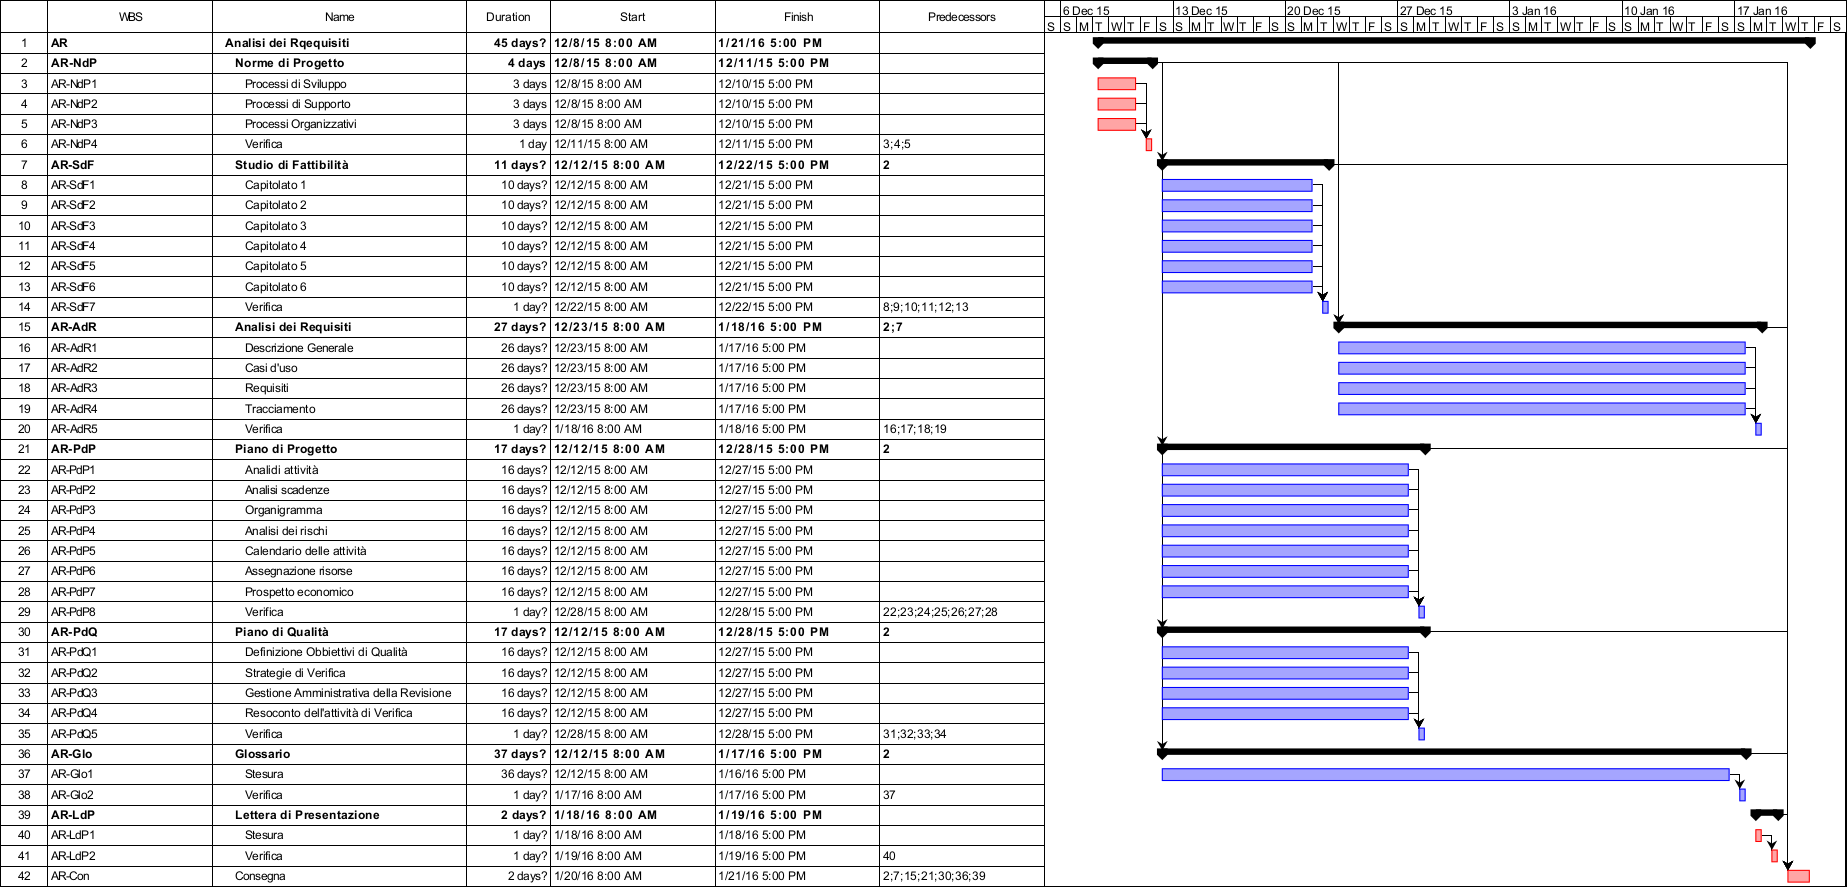
\includegraphics[keepaspectratio = true, width=23cm]{immagini/PdP_AnalisiDeiRequisitiGantt.png}
	\caption{Diagramma di \textit{Gantt\ped{G}} relativo al periodo di \AR.}\label{etichetta}
\end{sidewaysfigure}
\newpage

\subsubsection{\AD}
\textbf{Periodo:} dal 2016-01-23 al 2016-02-22. \\
Il periodo di \AD inizia subito dopo la consegna dei documenti per la \RR e termina con l'inizio del periodo successivo, quello della \PA. Il termine fissato corrisponde ad una \textit{milestone\ped{G}} interna. \\
In questo periodo il gruppo mira a consolidare ed ampliare i requisiti richiesti dal sistema e a migliorare il documento di \textit{\AdR} attuando le correzioni in base all'esito della \RR.
Vengono inoltre corretti e verificati anche gli altri documenti. 
In questa fase i ruoli maggiormente interessati sono quelli di \textit{\Ana} e \textit{\Ver}.  
\begin{center}
	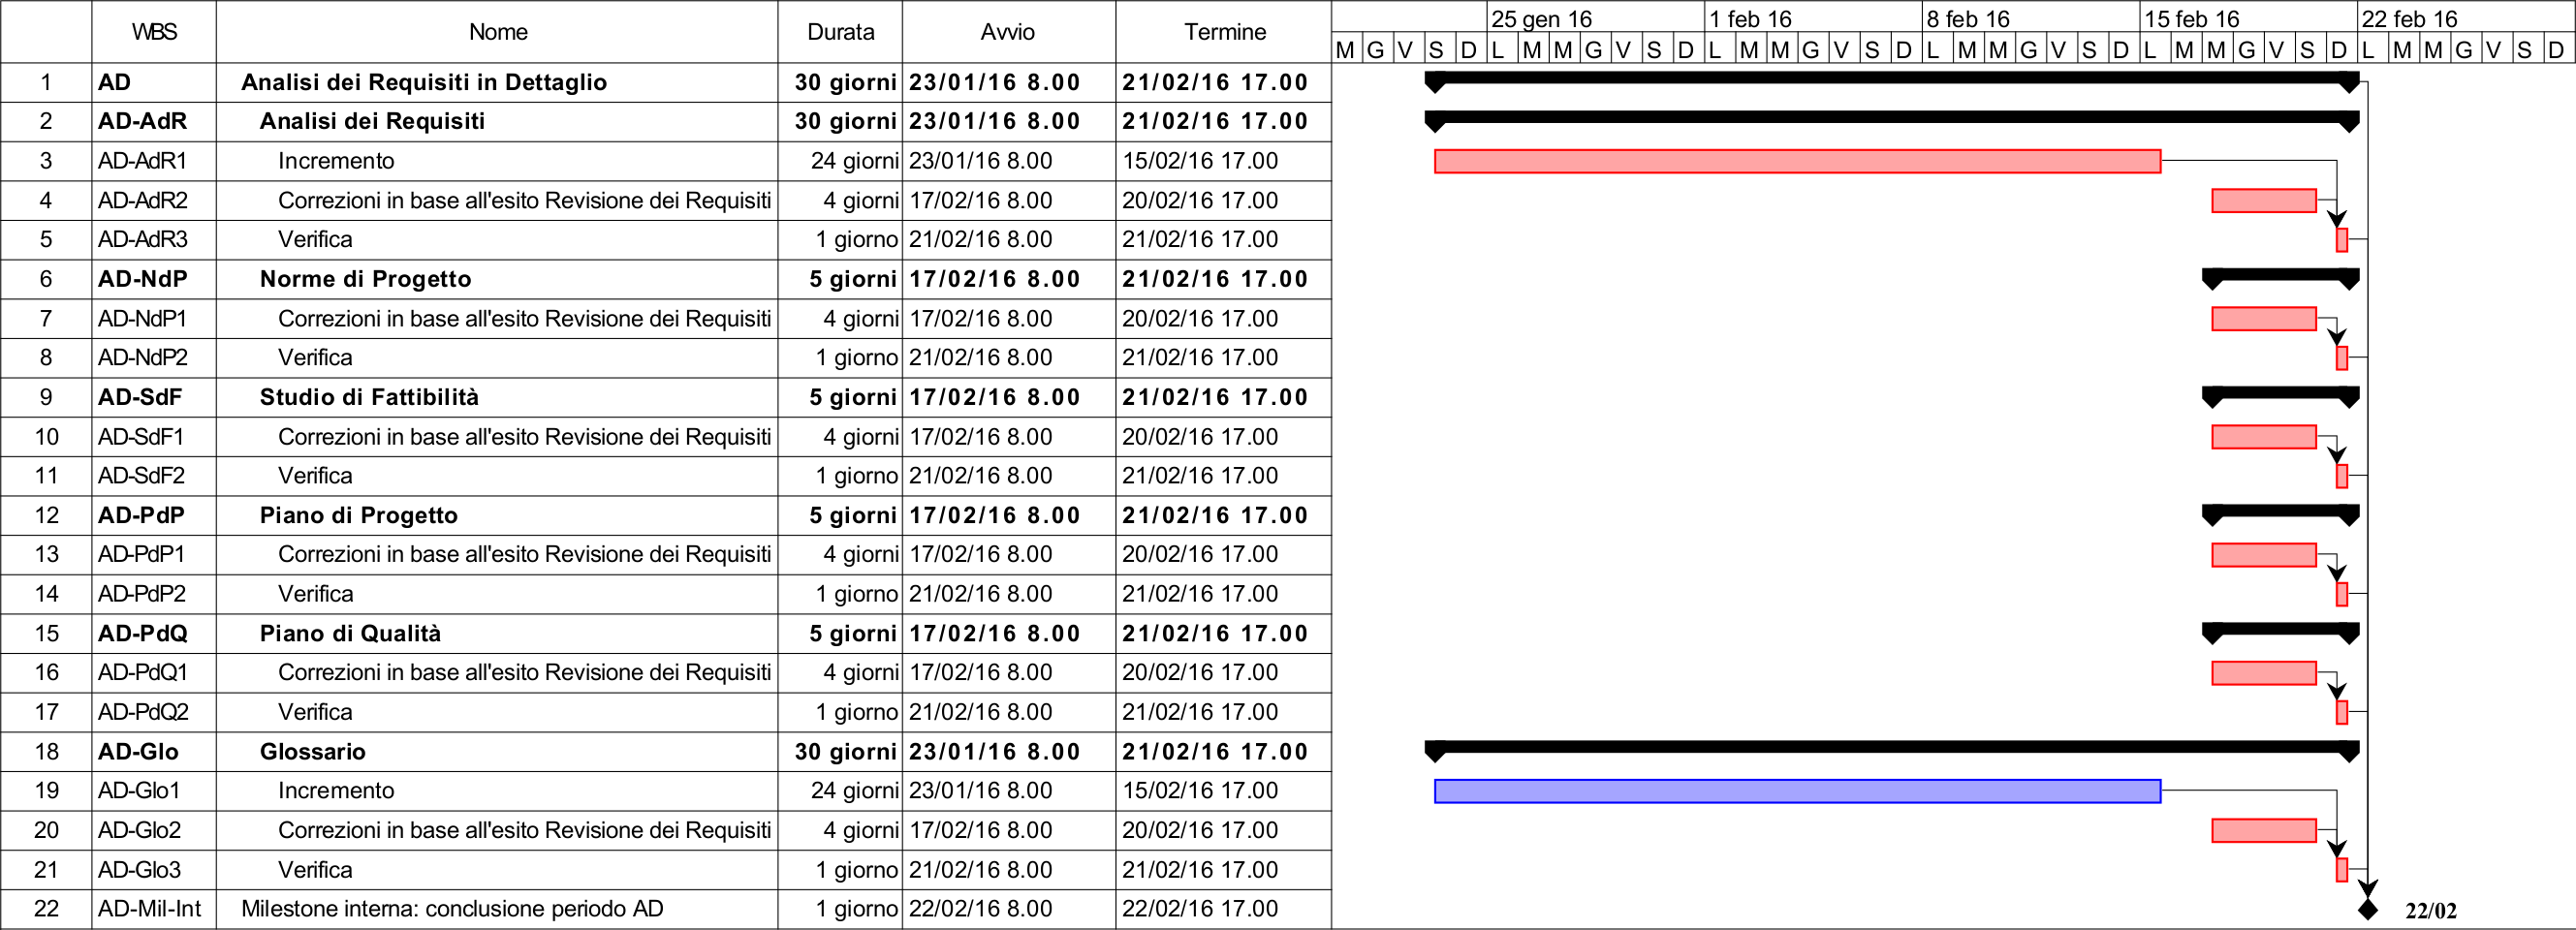
\includegraphics[keepaspectratio = true, width=16cm]{immagini/PdP_AnalisiDeiRequisitiInDettaglioGantt.png}
\end{center}
\begin{figure}[h]
	\caption{Diagramma di \textit{Gantt\ped{G}} relativo al periodo di \AD.}\label{etichetta}
\end{figure}

\subsubsection{\PA}
\textbf{Periodo:} dal 2016-02-23 al 2016-03-20. \\
Il periodo di \PA, inizia dopo quello di \AD e si conclude con una \textit{milestone\ped{G}} interna di \RdP minima. L'obbiettivo di questo periodo è la stesura della progettazione ad alto livello del sistema e prevede di svolgere le seguenti attività:
\begin{itemize}
	\item Redigere il documento di \textit{\ST}: il \textit{\Prog} deve descrivere le scelte progettuali di alto livello effettuate, i \textit{design pattern\ped{G}} scelti per la realizzazione del prodotto e l'architettura generale del software. Inoltre deve venir effettuato il tracciamento dei requisiti;  
	\item Incrementare i documenti di: \textit{\NdP},\textit{\PdP} e \textit{\PdQ};
	\item Verificare tutti i documenti sopraccitati.
\end{itemize}
In questa fase i ruoli maggiormente interessati sono quelli di \textit{\Amm}, \textit{\Res}, \textit{\Prog} e \textit{\Ver}. 
\begin{center}
	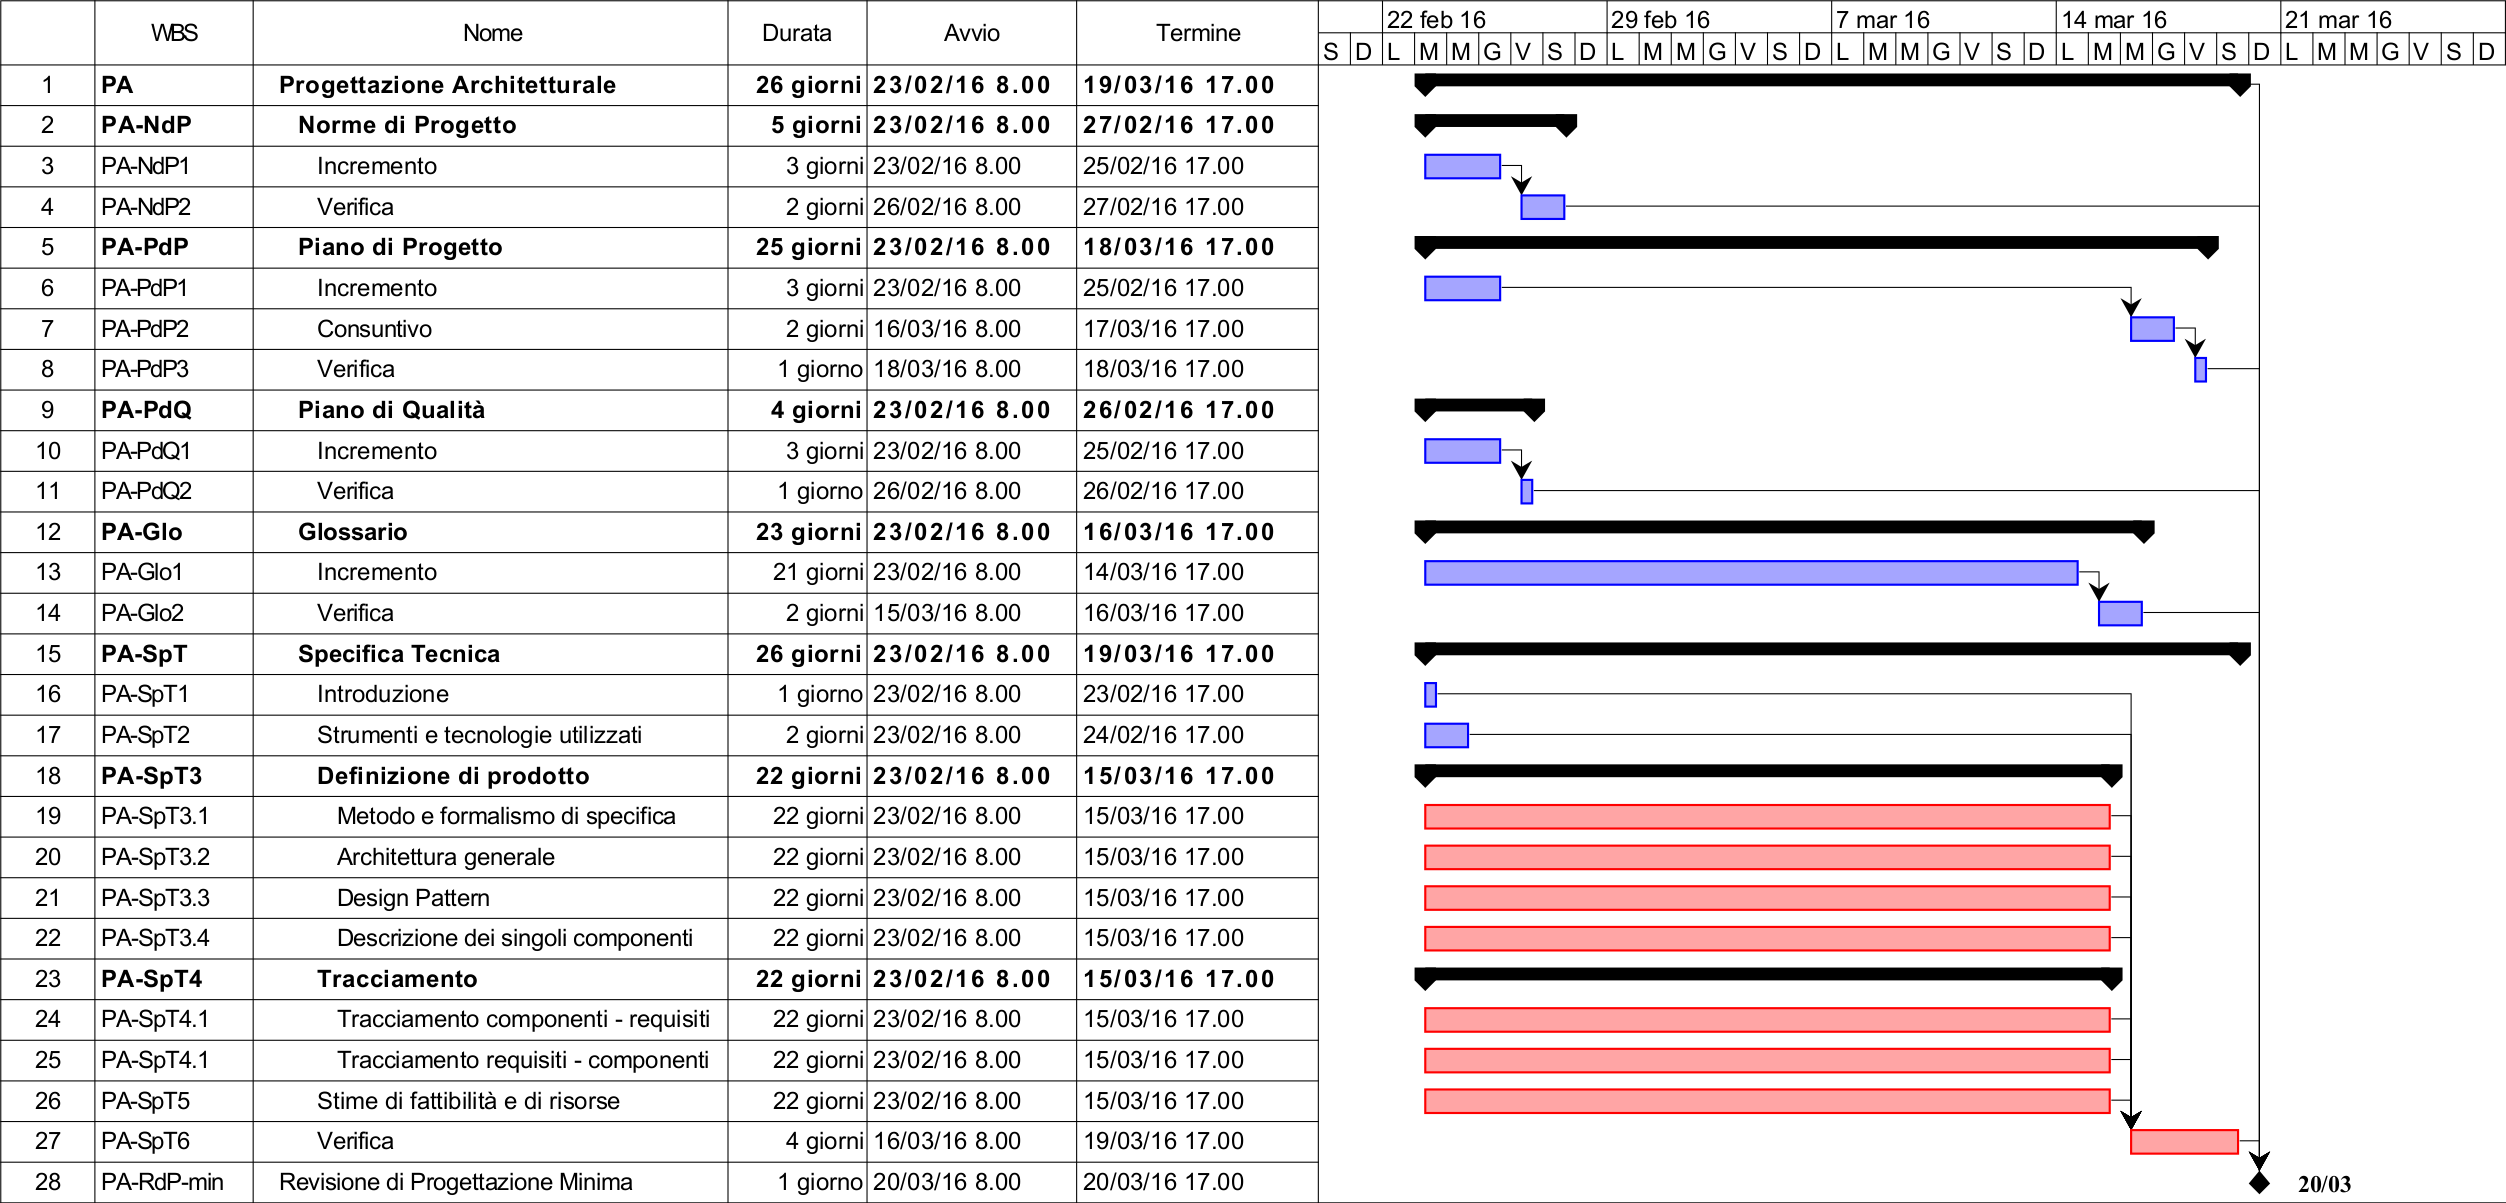
\includegraphics[keepaspectratio = true, width=16cm]{immagini/PdP_ProgettazioneArchitetturaleGantt.png}
\end{center}
\begin{figure}[h]
	\caption{Diagramma di \textit{Gantt\ped{G}} relativo al periodo di \PA.}\label{etichetta}
\end{figure}

\subsubsection{\PD}
\textbf{Periodo:} dal 2016-03-21 al 2016-04-11. \\
Il periodo di \PD, inizia dopo quello di \PA e si conclude con la consegna dei documenti per la \RP. L'obbiettivo di questo periodo è la stesura, in modo dettagliato, dell'intero sistema, specificando in modo approfondito il comportamento e l'iterazione tra i vari componenti. \\
Prevede di svolgere le seguenti attività:
\begin{itemize}
	\item Redigere il documento di \textit{\DDP}: il \textit{\Prog} deve descrivere il comportamento e le iterazioni tra i vari componenti del sistema basandosi sul documento di \textit{\ST};  
	\item Incrementare i documenti di: \textit{\NdP},\textit{\PdP}, \textit{\PdQ}, \textit{\ST} e \textit{\G};
	\item Verificare tutti i documenti sopraccitati.
\end{itemize}
In questa fase i ruoli maggiormente interessati sono quelli di \textit{\Amm}, \textit{\Res}, \textit{\Prog} e \textit{\Ver}. 
\begin{center}
	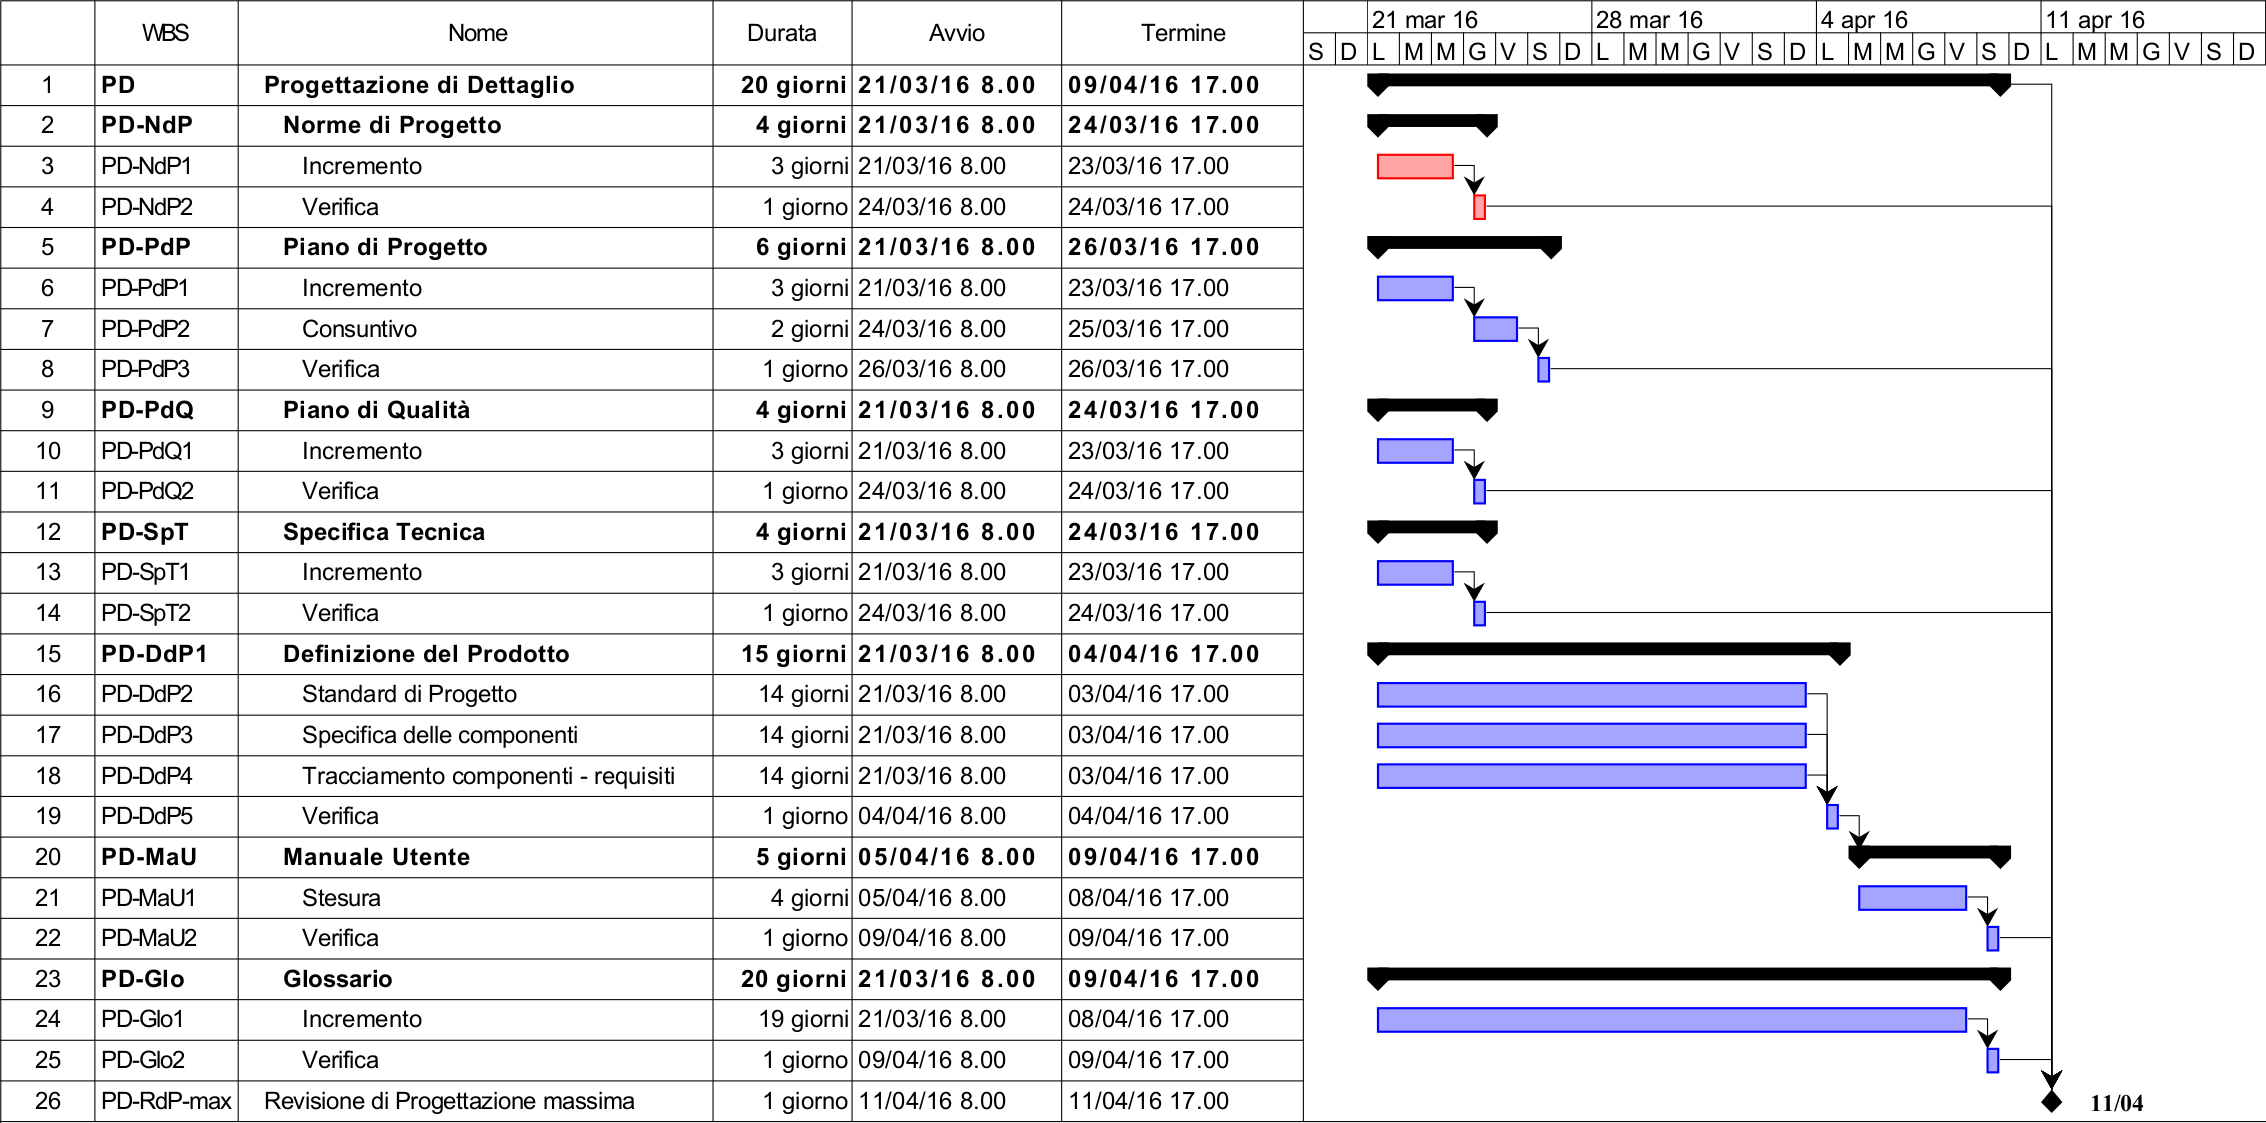
\includegraphics[keepaspectratio = true, width=16cm]{immagini/PdP_ProgettazioneDiDettaglioGantt.png}
\end{center}
\begin{figure}[h]
	\caption{Diagramma di \textit{Gantt\ped{G}} relativo al periodo di \PD.}\label{etichetta}
\end{figure}

\subsubsection{\CO}
\textbf{Periodo:} dal 2016-04-19 al 2016-05-16. \\
Il periodo di \CO, inizia dopo quello di \PD e si conclude con la consegna del prodotto alla \RQ. L'obbiettivo in questo periodo è di consegnare un prodotto qualificato e prevede di svolgere le seguenti attività:
\begin{itemize}
	\item \textbf{\CO}: attenendosi a quanto scritto dai \textit{\Progs} nel documento di \textit{\DDP}, i \textit{\Progrs} dovranno sviluppare il codice del prodotto software.\\
	L'attività di Codifica, dopo un primo momento, prevede due cicli incrementali per il miglioramento di parti del sistema esistenti o per l'aggiunta di funzionalità al sistema stesso. \\
	Ogni incremento prevede tre attività:
	\begin{itemize}
		\item Progettazione dell'incremento da parte dei \textit{\Progs};  
		\item Codifica da parte dei \textit{\Progrs} dell'incremento;
		\item Verifica dell'incremento. 
	\end{itemize}
	\item \textit{\MU}: documento destinato all'utilizzatore finale del prodotto che ne descrive le linee guida per il corretto utilizzo;
	\item Incrementare i documenti di: \textit{\NdP},\textit{\PdP}, \textit{\PdQ} e \textit{\G};
	\item Verificare tutti i documenti sopraccitati.
\end{itemize}
In questa fase i ruoli maggiormente interessati sono quelli di \textit{\Amm}, \textit{\Res}, \textit{\Prog}, \textit{\Progr} e \textit{\Ver}. 
\begin{center}
	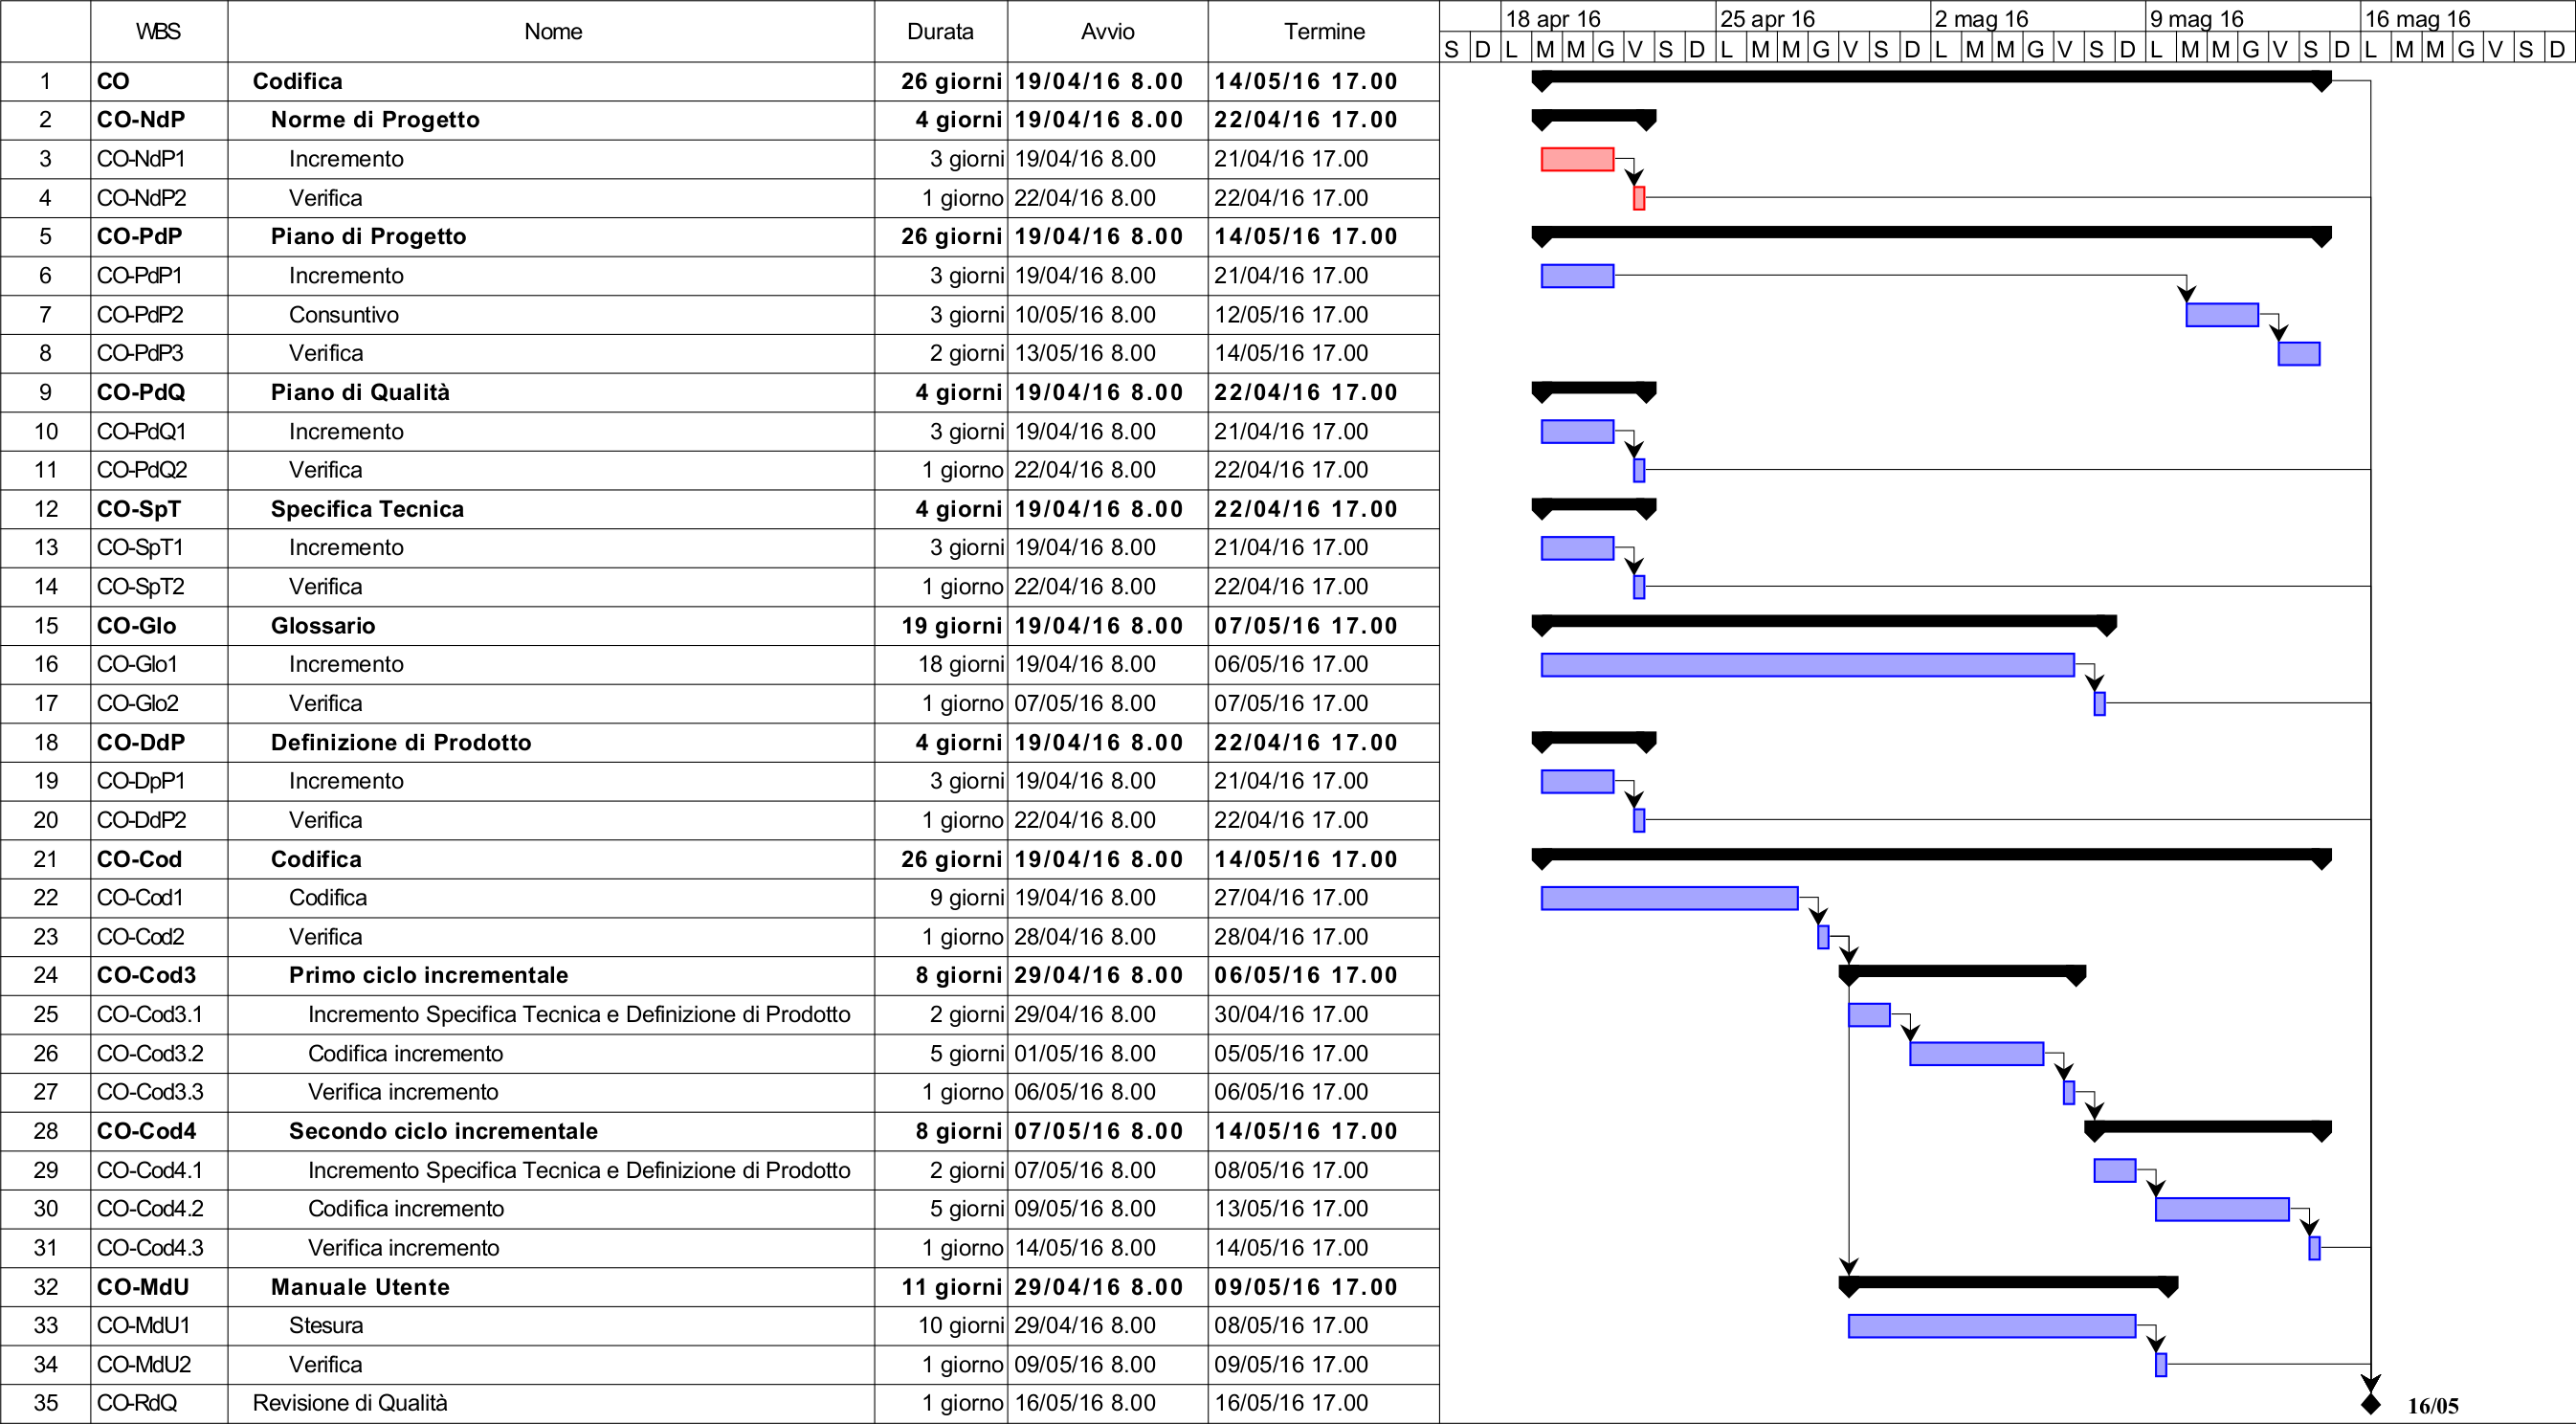
\includegraphics[keepaspectratio = true, width=16cm]{immagini/PdP_CodificaGantt.png}
\end{center}
\begin{figure}[h]
	\caption{Diagramma di \textit{Gantt\ped{G}} relativo al periodo di \CO.}\label{etichetta}
\end{figure}

\subsubsection{\VV}
\textbf{Periodo:} dal 2016-05-24 al 2016-06-10. \\
Questo periodo, di \VV, inizia dopo quello di \CO e si conclude con la consegna del prodotto alla \RA. In questo periodo vengono effettuati tutti i test necessari per garantire che il prodotto soddisfi tutti i requisiti dell'\AR.  
Le attività prevedono di:
\begin{itemize}
	\item Effettuare dei \textbf{test di sistema};  
	\item Incrementare i documenti di: \textit{\MU},\textit{\NdP},\textit{\PdP}, \textit{\PdQ} e \textit{\G};
	\item Verificare tutti i documenti sopraccitati.
\end{itemize}
In questa fase i ruoli maggiormente interessati sono quelli di \textit{\Res}, \textit{\Prog} e \textit{\Ver}. 
\newpage
\begin{center}
	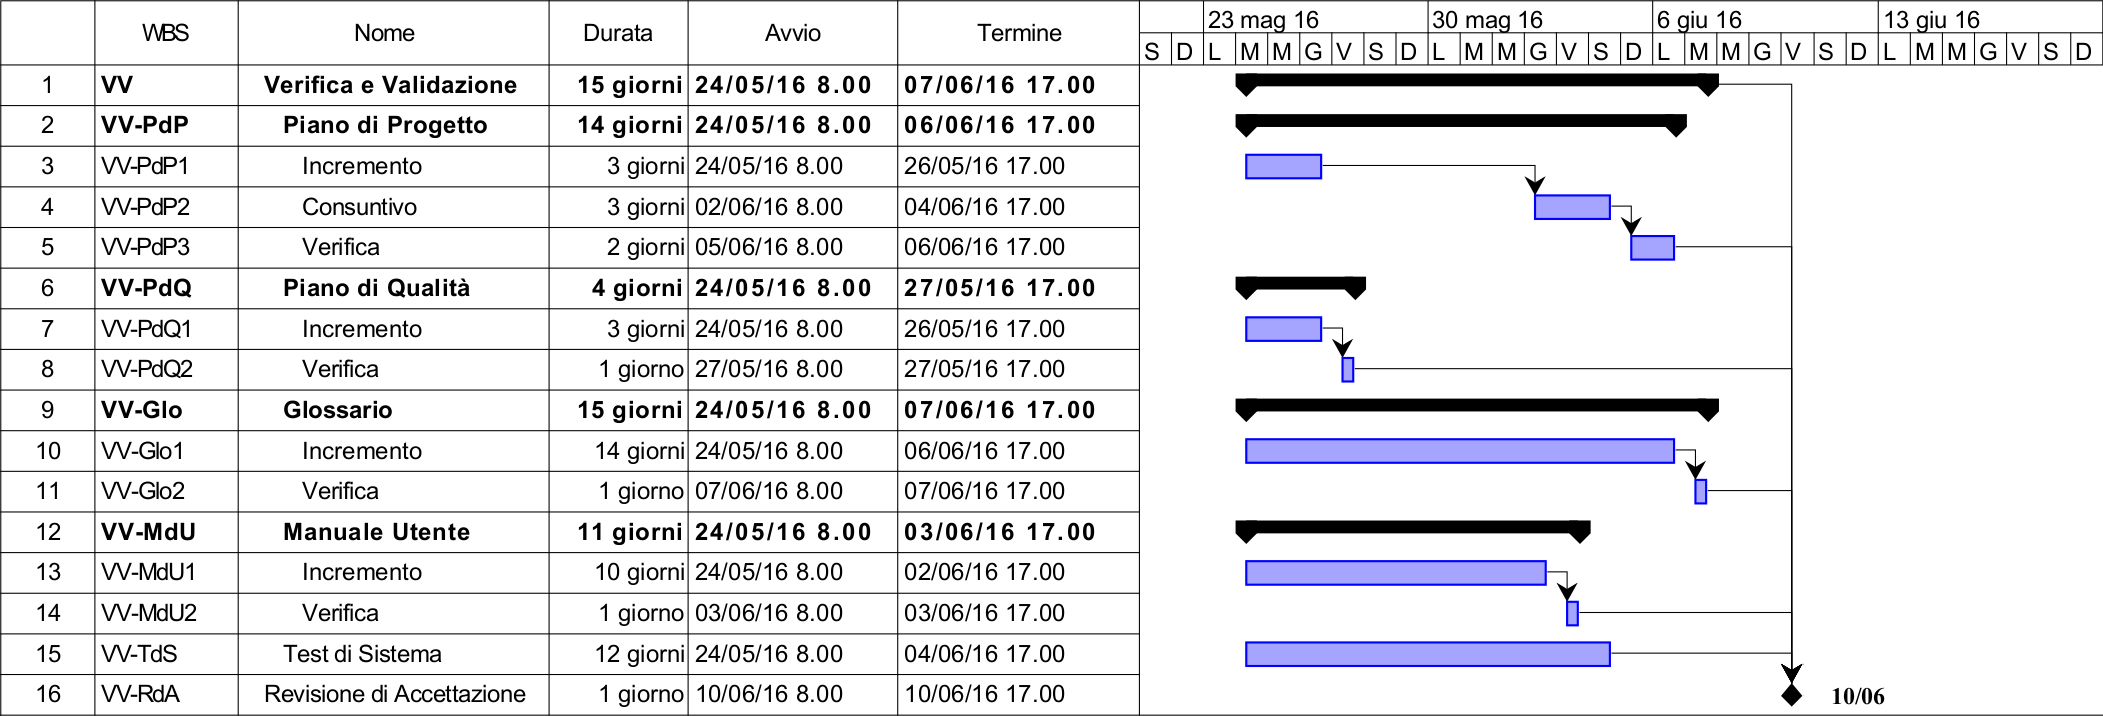
\includegraphics[keepaspectratio = true, width=16cm]{immagini/PdP_VerificaEValidazioneGantt.png}
\end{center}
\begin{figure}[h]
	\caption{Diagramma di \textit{Gantt\ped{G}} relativo al periodo di \VV.}\label{etichetta}
\end{figure}